This methodology involves generating a capable PINN model for the 2D-Difussion equation using a numerical method, and tensor flows. To begin, the diffusion equation is a partial differential equation that describes the spread of a quantity over time, given its initial distribution. In 2D, the diffusion equation is derived using the Green's functions \cite{Sukumar2022} and linear operator PDE's.  Guaranteed boundary conditions have to be specified in order to solve the diffusion equation. For this project both the Dirichlet's and Neumann's boundary conditions will be utilised \cite{Willis1980}. A neural network architecture is then chosen to approximate the solution to the diffusion equation. The neural network takes in the input variables $(x, y, t)$ and outputs the predicted value of $u(x,y,t)$ as an example. The architecture in Figure \ref{fig:arch} is designed based on the complexity of the problem and the available data. Following this we can use the PINNs technique to train the neural network. The PINN technique involves minimizing the difference between the predicted and actual values of the quantity of interest, as well as satisfying the differential equation and boundary conditions. This can be done using optimization algorithms such as stochastic gradient descent, sequential or adam \cite{FernandezdelaMata2023}. Finally, after the neural network is trained, we can use it to predict the distribution of $u(x,y,t)$ function over time. We can then use data visualization techniques such as contour plots or surface plots to visualize the predicted distribution. 
\begin{figure}[htb!]
\begin{center}
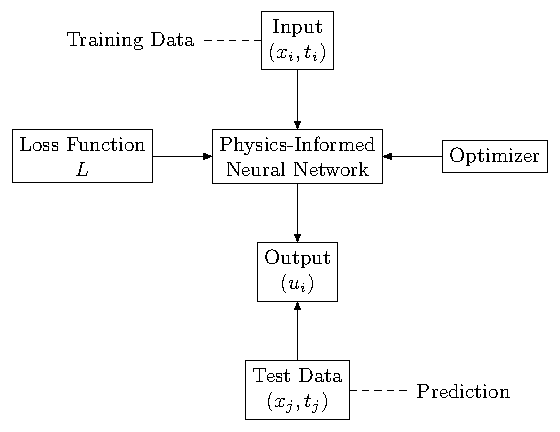
\includegraphics[width=.49\textwidth]{images/arc.pdf}
\vspace*{-8mm}
\caption{PINNs Architecture}
\label{fig:arch}
\end{center}
\end{figure}

During training, the PINN model should satisfy the 2D Diffusion equations as a constraint, and the generated data set should be used to compute the loss function. As a result the performance of the PINN model will be evaluated in predicting the diffusivity using various metrics, such as mean absolute error, root mean square error, and or the correlation coefficient.

\subsection{Solution to the 2D Diffusion Equation}
The 2D diffusion equation allows us to talk about the statistical movements of randomly moving particles in two dimensions. The movement of each individual particle does not follow the equation, but many identical particles each obeying the same boundary and initial conditions share some statistical properties. In this derivation of the diffusion PDE we well use function $P$ instead of $U$ to easily set apart the derivation function from the function used in the code section even though they mean the same. 
In an ideal world the diffusion function is just the probability distribution $P(x,y,t)$ which provides the probability of finding a perfectly average particle in the small vicinity of the point $(x,y$) at a given time $t$. The Brownian motion is a special case of diffusion 2D where the particles are subject to random forces that cause them to move in a random pattern \cite{Ursell2005}. The movement of particles in both diffusion 2D and Brownian motion is affected by the diffusion coefficient $D$, which represents the degree of randomness in the movement of the particles. The evolution of some systems does follow the equation outright but as a group they exhibit the smooth, well-behaved statistical features of the diffusion equation.

Now that with all the relative background knowledge, let's start with the 2D diffusion equation in cartesian coordinates as:
\begin{align*}
    \nabla^2 - \frac{1}{D} \frac{\partial P}{ \partial t} = 0 \\
    \frac{\partial^2 P}{ \partial^2 x^2} + \frac{\partial^2 P}{ \partial^2 y^2}  - \frac{1}{D} \frac{\partial P}{ \partial t} = 0 \tag{1}
    \label{eq1}
\end{align*}

Equation \eqref{eq1} is what we're interested in, but in order to solve it we will need to define the boundary conditions as follows:

\begin{align*}
   \frac{\partial^2 P}{\partial x^2} \bigg \vert_{x = \pm -\infty} = \frac{\partial^2 P}{\partial y^2} \bigg \vert_{y= \pm \infty} &= 0 \\
   \frac{\partial P}{\partial x} \bigg \vert_{x= \pm \infty} = \frac{\partial P}{\partial y} \bigg \vert_{y= \pm \infty} &= 0 \tag{B.C}
    \label{bc1}
\end{align*}

Since the function $P$ is a linear partial differential equation and separable function, we can apply an inverse 2D Fourier transform to solve the solution. Consider the following integral relations that define the 2D FT in Cartesian coordinates. We will call the function $\hat{P}$ the FT of our original function $P$:

\begin{align*}  
  \hat{P}(k_x,k_y,t) =  \oiint_{s} e^{-i 2\pi (k_x \cdot x + k_y \cdot y )} P(x,y,t) dx dy \\  
  P(x,y,t) = \oiint_{s} e^{-i 2\pi (k_x \cdot x + k_y \cdot y )} \hat{P}(k_x,k_y,t) dx dy \tag{2}
  \label{eq2}  
\end{align*}  

Notice the symmetry in going forward and backward in the transform Equation \eqref{eq2}. This is because switching between the normal form of the problem and what we call Fourier Space, where the problem exists after the FT, are physically identical. Let’s examine the spatial derivatives of the diffusion equation, where we consider the second derivative to be the function of interest. We can integrate these second derivatives by parts, using $u$ and $v$ as follows:
\begin{align*}  
\int\limits_{a}^{b} udv = uv \bigg \vert^{b}_{a} - \int\limits_{a}^{b} vdu 
\label{ibp1}  
\end{align*} 
\twocolumn[\begin{@twocolumnfalse}
\begin{align*} 
\textnormal{ if } u = e^{-i 2\pi (k_x \cdot x + k_y \cdot y )} \textnormal{ and } v &= \frac{\partial P}{\partial x} \\
\textnormal{ then } du= \frac{\partial}{\partial x} e^{-i 2\pi (k_x \cdot x + k_y \cdot y )} \textnormal{ and } dv &=  \frac{\partial^2 P}{\partial x^2} dx
\label{ibp2}  
\end{align*}  

Using the substitution of integration by parts we can set up the whole integral as follows.

\begin{align}  
% \iint\limits_{-\infty}^{\infty} e^{-i 2\pi (k_x \cdot x + k_y \cdot y )} \hat{P}(k_x,k_y,t) dx dy \tag{5} \\
\integral e^{-i 2\pi (k_x \cdot x + k_y \cdot y )} \frac{\partial^2 P}{\partial x^2} dx dy &= e^{-i 2\pi (k_x \cdot x + k_y \cdot y )} \frac{\partial P}{\partial x} \bigg \vert^{\infty}_{-\infty(x,y)} - \integral \frac{\partial }{\partial x} e^{-i 2\pi (k_x \cdot x + k_y \cdot y )} \cdot \frac{\partial P}{\partial x} dx dy\\
& = e^{-i 2\pi (k_x \cdot x + k_y \cdot y )} \frac{\partial P}{\partial x} \bigg \vert^{\infty}_{-\infty(x,y)} + i 2\pi k_x \integral e^{-i 2\pi (k_x \cdot x + k_y \cdot y )} \frac{\partial P}{\partial x} \\
& = \cancel{e^{-i 2\pi (k_x \cdot x + k_y \cdot y )} \frac{\partial P}{\partial x} \bigg \vert^{\infty}_{-\infty(x,y)}} + i 2\pi k_x \integral e^{-i 2\pi (k_x \cdot x + k_y \cdot y )} \cdot \frac{\partial P}{\partial x} dx dy\\
& = i 2\pi k_x \integral e^{-i 2\pi (k_x \cdot x + k_y \cdot y )} \frac{\partial P}{\partial x} \tag{3}
\label{eq3}  
\end{align}  

Looking the last term Equation \eqref{eq3}, we effectively transferred one derivative off $P$ and put it on the exponential of the FT, but since the exponential is an explicit function we can just perform the derivative, giving us the constant on the right most integral of the second line. We can apply similar inverse 1D Fourier transform Equation \eqref{eq3} again to get:

\begin{align}  
\integral e^{-i 2\pi (k_x \cdot x + k_y \cdot y )} \frac{\partial P}{\partial x} dx dy &= P \cdot e^{-i 2\pi (k_x \cdot x + k_y \cdot y )} \bigg \vert^{\infty}_{-\infty(x,y)} - \integral \frac{\partial }{\partial x} e^{-i 2\pi (k_x \cdot x + k_y \cdot y )} \cdot P \cdot dx dy\\
& = \cancel{P \cdot e^{-i 2\pi (k_x \cdot x + k_y \cdot y )} \bigg \vert^{\infty}_{-\infty(x,y)}} + i 2\pi k_x \integral P \cdot e^{-i 2\pi (k_x \cdot x + k_y \cdot y )} dx dy\\
& = i 2\pi k_x \integral e^{-i 2\pi (k_x \cdot x + k_y \cdot y )} dx dy \tag{4}
\label{eq4}  
\end{align} 

Equating all the L.H.S with the R.H.S Equation \eqref{eq4} we get: 

\begin{align}  
\integral e^{-i 2\pi (k_x \cdot x + k_y \cdot y )} \frac{\partial^2 P}{\partial x^2} dx dy &= (i 2\pi k_x)^2 \integral e^{-i 2\pi (k_x \cdot x + k_y \cdot y )} dx dy \\
\integral e^{-i 2\pi (k_x \cdot x + k_y \cdot y )} \frac{\partial^2 P}{\partial x^2} dx dy &= (i 2\pi k_x)^2 \hat{P} \tag{5}
\label{eq5}  
\end{align} 

Since we took the spatial FT (i.e. dealing with x and y), keep in mind, the derivative in time does not change under a FT \cite{TANG2022186}. Henceforth we can write the 2D Equation \eqref{eq5} as follows, that enable us to use method of separation variables for an Eigen value problem in resulting Equation \eqref{eq6}: 

    \begin{align*}
     % \textnormal{ This generally corresopnds to the format } \\
    \frac{\partial^n}{\partia x^n} = (i 2\pi k_x)^n \hat{P} \\
    % \textnormal{ This means the equation becomes first order ODE in time: } \\
    (2\pi)^2 \hat{P} \cdot ((k_x)^2 + (k_y)^2)  + \frac{1}{D} \frac{\partial P}{ \partial t}=0\\
    \hat{P} = \lambda e^{-D (2\pi)^2 (k_x^2 + k_y^2) \cdot t} \tag{6}
    \label{eq6}   
    \end{align*}    

\end{@twocolumnfalse}]
\twocolumn[\begin{@twocolumnfalse}

The constant $\lambda$ is nothing but the normalization factor that can be used for the conservation of linear momentum \cite{Ursell2005}. Therefore our original function $p$ is then given by:

\begin{align*}
    P &=\lambda\integral e^{-D (2\pi)^2 (k_x^2 + k_y^2) t}\cdot e^{-i 2\pi (k_x \cdot x + k_y \cdot y )}dk_x dk_y \tag{7}
    \label{eq7}  
\end{align*}

We can further compute Equation \eqref{eq7} by method of separation of spatial variable as:

\begin{align*}
    P &= \lambda \int\limits^{\infty}_{\text{-}\infty} e^{i 2\pi k_x \cdot x-D (2 \pi k_x)^2 t}dk_x \cdot \int\limits^{\infty}_{\text{-}\infty} e^{-i 2\pi k_y \cdot y-D (2 \pi k_y)^2 t}dk_y  \\
    P &= \lambda \left\{ \int\limits^{\infty}_{\text{-}\infty} e^{i 2\pi k_x \cdot x-D (2 \pi k_x)^2 t}dk_x \right \} \cdot  \left\{ \int\limits^{\infty}_{\text{-}\infty} e^{-i 2\pi k_y \cdot y-D (2 \pi k_y)^2 t}dk_y \right \} \tag{8}
    \label{eq8}  \\
\end{align*}

Solving Equation \eqref{eq8} by separation of integral requires completing the square of the exponent, re-scaling the integration variable, changing to polar coordinates and then substituting back the Cartesian values. We will look at the integrand part of each individual section first.  

% \begin{center}
  \begin{align}
    P &= \lambda \int\limits^{\infty}_{\text{-}\infty} e^{\underbrace{i 2\pi k_x \cdot x-D (2 \pi k_x)^2 t}_{\text{1}}dk_x} \cdot \int\limits^{\infty}_{\text{-}\infty} e^{\underbrace{i 2\pi k_y \cdot y-D (2 \pi k_y)^2 t}_{\text{2}}dk_y}
\end{align} 
\begin{align}
    \underbrace{i 2\pi k_x \cdot x-D (2 \pi k_x)^2 t}_{\text{completing square for 1}} &= -4 \pi^2 D t \bigg(k_x -\frac{ix}{2 \pi D t}\bigg)^2 - \frac{x^2}{4 D t} \\
    \textnormal{ Let } u_x &= k_x -\frac{ix}{2 \pi D t} \textnormal{ then }\\
      &= -4 \pi^2 D t u_x^2 - \frac{x^2}{4 D t}\\  
    \int\limits^{\infty}_{\text{-}\infty} e^{\underbrace{i 2\pi k_x \cdot x-D (2 \pi k_x)^2 t}_{\text{1}}dk_x} &= e^{\frac{-x^2}{4 D t}}\int\limits^{\infty}_{\text{-}\infty} e^{4 \pi^2 D t \cdot u_x^2 du_x} \tag{9}
    \label{eq9}\\
\end{align}  
Similarly for the second section of the equation we have:
  \begin{align}  
    \underbrace{i 2\pi k_y \cdot y-D (2 \pi k_y)^2 t}_{\text{completing square for 2}} &= -4 \pi^2 D t \bigg(k_y -\frac{iy}{2 \pi D t}\bigg)^2 - \frac{y^2}{4 D t} \\
    \textnormal{ Let } v_x &= k_y -\frac{iy}{2 \pi D t} \textnormal{then} \\
      &= -4 \pi^2 D t v_x^2 - \frac{y^2}{4 D t} \\  
    \int\limits^{\infty}_{\text{-}\infty} e^{\underbrace{i 2\pi k_y \cdot x-D (2 \pi k_y)^2 t}_{\text{2}}dk_y} &= e^{\frac{-y^2}{4 D t}}\int\limits^{\infty}_{\text{-}\infty} e^{4 \pi^2 D t \cdot v_x^2 dv_x} \tag{10}
    \label{eq10}
\end{align} 

After dividing the equation in to two sections, we will attempt to solve each one individually beginning with the first section obtained in Equation \eqref{eq9}. \\
\end{@twocolumnfalse}]

Notice, Equation \eqref{eq9} is equivalent to the first integral in the original expression, up to a constant factor of $e^{-x^2/(4 D t)}$ with a non elemental integral on the integrand \cite{conradB}. To solve this equation we will need to use substitution and then changing to polar coordinates.

Let $$ v =2\pi \sqrt{D t} \cdot u_x$$ then:

\begin{align*}
    \int\limits^{\infty}_{\text{-}\infty} e^{4 \pi^2 D t \cdot u_x^2 dU_x} &= \int\limits^{\infty}_{\text{-}\infty} e^{\frac{-v^2}{4}dv} \tag{11}
    \label{eq11}
\end{align*}

The integral in Equation \eqref{eq11} can be evaluated using the standard result and method of re-scaling as:
$$ \int\limits^{\infty}_{\text{-}\infty} e^{-x^2/2} dx = \sqrt{2\pi} $$

To see why, we can consider the square of this integral and evaluate it in polar coordinates: 

\begin{center}
\begin{equation*}
    \begin{rcases}
        $$x = r\cos \theta$$ \\
        $$y = r\sin \theta$$ \\
        $$x^2 + y^2 = r^2$$ \\
        $$dxdy = rdrd \theta$$\\
    \end{rcases}
    \text{polar transformation}  
\end{equation*}
\end{center}

\begin{align*}
\left(\int_{-\infty}^{\infty} e^{-x^2/2} dx\right)^2  &= \int\limits^{\infty}_{\text{-}\infty} e^{-x^2/2} dx \cdot \int\limits^{\infty}_{\text{-}\infty} e^{-y^2/2} dy \\
&= \integral e^{-x^2/2} \cdot e^{-y^2/2} dx dy \\
&= \integral e^-{\frac{x^2 + y^2}{2}} dx dy \\
&= \int_{0}^{2\pi} \int_{0}^{\infty} e^{-r^2/2} \cdot r dr d\theta \\
&= 2\pi \int_{0}^{\infty} e^{-r^2/2} r dr \\
&= -2\pi \left[e^{-r^2/2}\right]_{0}^{\infty} \\
&= \left(\sqrt{2\pi}\right)^2 \tag{12}
\label{eq12}
\end{align*}

Therefore from Equation \eqref{eq12} we have:

\begin{align*}
\int\limits^{\infty}_{\text{-}\infty} e^{-4 \pi^2 D t u_x^2} du &= \int\limits^{\infty}_{\text{-}\infty} e^{-v^2/4} dv \\
&= 2 \int\limits^{\infty}_{0} e^{-v^2/4} dv  \\
&= 2\sqrt{\pi} \tag{13}
\label{eq13}
\end{align*}

Substituting $v$ from Equation \eqref{eq11} back to in Equation \eqref{eq9} and multiplying both by $e^{-x^2/(4Dt)}$, we obtain:

\begin{align*}
e^{-\frac{x^2}{4Dt}} \int_{-\infty}^{\infty} e^{-4 \pi^2 D t u^2} du &= \sqrt{\frac{\pi}{4Dt}}\, e^{-\frac{x^2}{4Dt}} \tag{14}
\label{eq14}
\end{align*}


Now remember this is only for the Left ($dk_x$) section of Equation \eqref{eq9}. We still need to follow the same process for the Right ($dk_y$) section in Equation \eqref{eq10}. Following the same process we obtain Equation \eqref{eq15} as: 

\begin{align*}
e^{-\frac{y^2}{4Dt}} \int_{-\infty}^{\infty} e^{-4 \pi^2 D t v^2} dv &= \sqrt{\frac{\pi}{4Dt}}\, e^{-\frac{y^2}{4Dt}} \tag{15}
\label{eq15}
\end{align*}

Finally putting all equations together and multiplying the two sections in Equation \eqref{eq8} we have: 
\begin{align*}
    P(x,y,t) = \lambda \frac{e^{\frac{-(r^2)}{4 D t}}}{4 \pi D \cdot t} \tag{polar} \\
    P(x,y,t) = \lambda \frac{e^{\frac{-(x^2 + y^2)}{4 D \cdot t}}}{4 \pi D t} \tag{16} 
    \label{eq16}  
\end{align*}
One last step is to figure out what $\lambda$ exactly is in Equation \eqref{eq16}. For this sample of project the normalization constant $\lambda$ is just the sum unity function that represents the total sum of the diffusive particles across the 2D surface in the Gaussian distribution. So on larger scales the trainable degrees of freedom behave as Gaussian random variables and on somewhat smaller scales the dynamics is frustrated from the simultaneous maximization of entropy of non-trainable variables and minimization of entropy of trainable variables \cite{Katsnelson2023}. These results have some interesting implications for machine learning and physics. So the constant essentially tells us how many non-interacting particles we have in the system (we are considering just one representative particle). Thus, if we apply the boundary condition from $-\infty$ to $+\infty$, the total sum of the function $P (x,y,t)$ adds up to $1$. Imposing this condition leads us to Equation \eqref{eq17}: 
\begin{align*}
    \lambda = \integral P(x,y,t) dx dy= 1 \tag{17}
    \label{eq17}  
\end{align*}

There for, if $\lambda = 1$ the entirety of the 2D diffusion equation results to Equation \eqref{eq18}: 

\begin{align*}
    \boxed{
    P(x,y,t) = \frac{e^{\frac{-(x^2 + y^2)}{4 D \cdot t}}}{4 \pi D t} \tag{18} }
    \label{eq18}  
\end{align*}
A detailed complete PDE derivation of the solution to the diffusion 2D problem can be found here \cite{Eyob2023}. 


\subsection{Code Setup}
The code for this project tries to demonstrate how to use a neural network in order to solve thee diffusion equation. The main diffusion equation as shown in Equation \eqref{eq18} is defined in the code by the function "diffusion\_equation", which takes in the position, time, and diffusion coefficient as inputs and returns the value of the equation at that point as seen in the code below. Here the $\lambda$ constant is set to 1 and the cartesian form of the function provided in Equation \eqref{eq17} is utilised. The domain and boundary conditions for the problem are defined by creating a grid of x and t values using the NumPy meshgrid function. The model is built using the Keras Sequential API and consists of three fully connected layers, with the output layer having a linear activation function. The model is trained using mean squared error loss and the RMSprop optimizer. Finally, the model is used to predict the diffusion equation for each value of D, and the results are plotted using the Matplotlib library. Full codes to the project can be found on github \cite{Eyob2023_Git}.

\begin{center}
   \begin{verbatim}
    # This is the main Diffusion equation
    def diffusion_equation(x, t, D):
      return 1 / (4 * np.pi * D * t) * 
      np.exp(-np.linalg.norm(x) ** 2 / (4*D*t))

    # Applying boundary conditions
    x = np.linspace(-1, 1, 50)
    t = np.linspace(0.01, 1, 20)
    X, T = np.meshgrid(x, t)
    X_flat = X.flatten()
    T_flat = T.flatten()
    D_values = [0.1, 0.2, 0.3, 0.4]
    N = X_flat.shape[0]
\end{verbatim} 
\end{center}


Based on the code provided above, one can observe that the model is trained to predict the values of the diffusion equation at different points in space and time, for a range of diffusion coefficients. The training process involved minimizing the difference between the predicted values and the actual values of the diffusion equation using mean squared error loss. 

After training, the model is used to predict the values of the diffusion equation for each value of the diffusion coefficient in the range of D\_values. The predicted values are then plotted using contour plots, with the x-axis representing position, the y-axis representing time, and the color indicating the value of the diffusion equation.

As stated in the methods section, the homogeneous Neumann's boundary conditions are assumed (refer to the \eqref{bc1}). These boundary conditions state that the normal derivative of the solution at the boundary is zero. In this code, the boundaries of the domain are implicitly assumed to be reflective, which means that the diffusion equation at the boundaries is equal to zero. This assumption is necessary to avoid numerical errors due to the finite size of the domain.
 
% There for we will use the Equation (\ref{eq15}) as our main equation for the  PiNN's model. 